% Chapter 5

\chapter{Evaluation} % Main chapter title
\label{Chapter5} % For referencing the chapter elsewhere, use \ref{Chapter5} 

\lhead{Chapter 5. \emph{Evaluation}} % This is for the header on each page - perhaps a shortened title
%----------------------------------------------------------------------------------------
In this section we discuss the evaluation of design and implementation of the work done in this thesis. We conduct feature evaluations and performance experiments on the prototype implementation of discussed solution components in specific experiment setups in order to derive conclusions.
\section{Feature Evaluation Aspects}
\subsection{Functional coverage}
The proposed solution should be able to deal with the standard open data preparation processes including data cleaning and RDF creation. We did a comparative analysis with the features supported by Grafter which was previously used to perform open data preparation, to ensure functional coherence and coverage of newly implemented system.  The prototype as of now supports following features in distributed computing manner and exposed to users using a DSL abstraction which is supported by dynamic transformation execution engine (Scalable-graftwerk). 
\begin{center}
	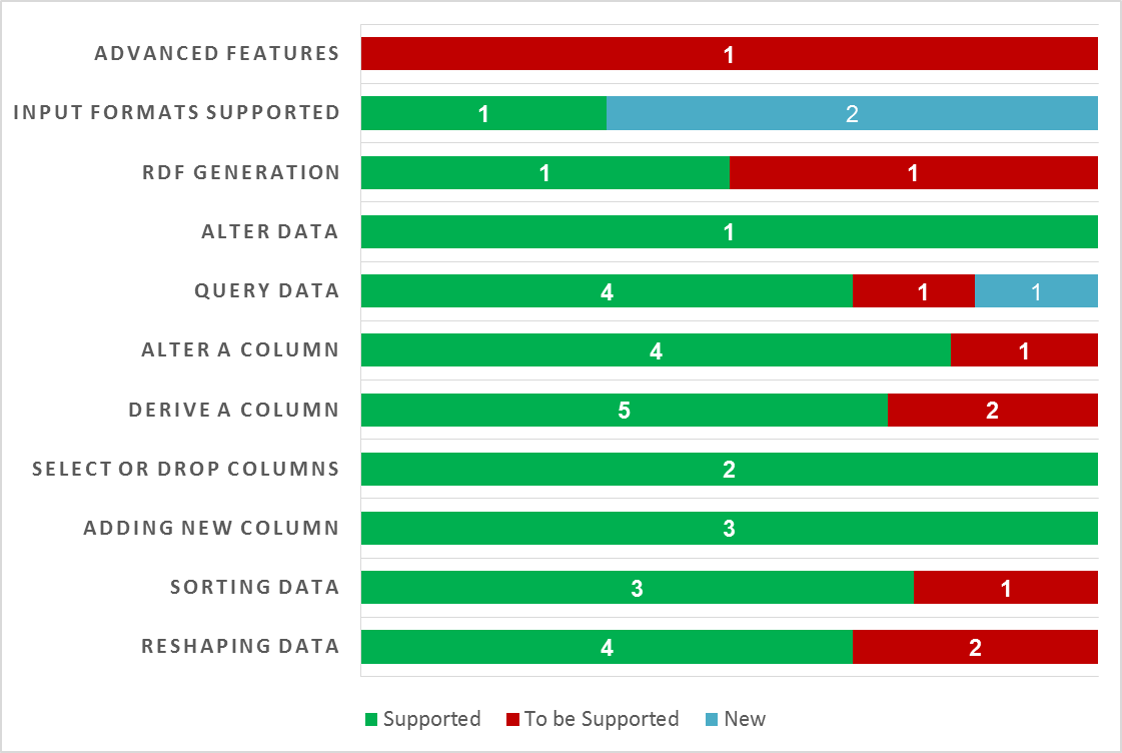
\includegraphics[width=38em]{./Figures/functional-coverage-new}
	\begin{figure}[htbp]
    \caption{Functional coverage of Scalable-graftwerk}
    \label{fig:func-coverage}
	\end{figure}
\end{center}
 In summary, implemented solution provides 39/47 major operations, i.e, ( ~83\% ), of requirements. Figure \ref{fig:func-coverage} shows that, most of the data cleaning functions are covered by implemented prototype as well as it can create RDF formats using simple mapping. In addition, Sparker provides more features such as querying using common logical expressions and supports more input formats.   Currently, it mainly lacks support of user-defined implementations of cleaning operations and pipeline functions due to the newly introduced context of distributed cleaning operations. However, provided that the main purpose of this solution is to support a user friendly, interactive data preparation, that can help to engage marginal audience in open data preparations, the currently implemented features satisfy user's requirements. 
% % how many implemented n wht is missing
% \subsection{Accuracy and consistency}
% how sampling helps? how consistent are sample n full execution vs other systems execution

\subsection{User friendliness}
User friendliness and a general purpose data preparation solution are important requirements of this solution. It is important to measure the user friendliness that is provided by the tool as it is expected to be used by users with various technical background. Grafterizer provides a very simple, easily understandable and intuitive interface with well explained documentation for  data cleaning and visualization, whereas other solutions such as Wrangler\cite{2011-wrangler}\cite{openrefine} require user to use domain-specific scripting to perform relevant data cleaning. This implicitly requires at least moderate level of technical knowledge which can be comparably tedious, time consuming and error prone. The user can use user interfaces in Grafterizer to perform data cleaning without manually entering cleaning scripts. 
\begin{center}
	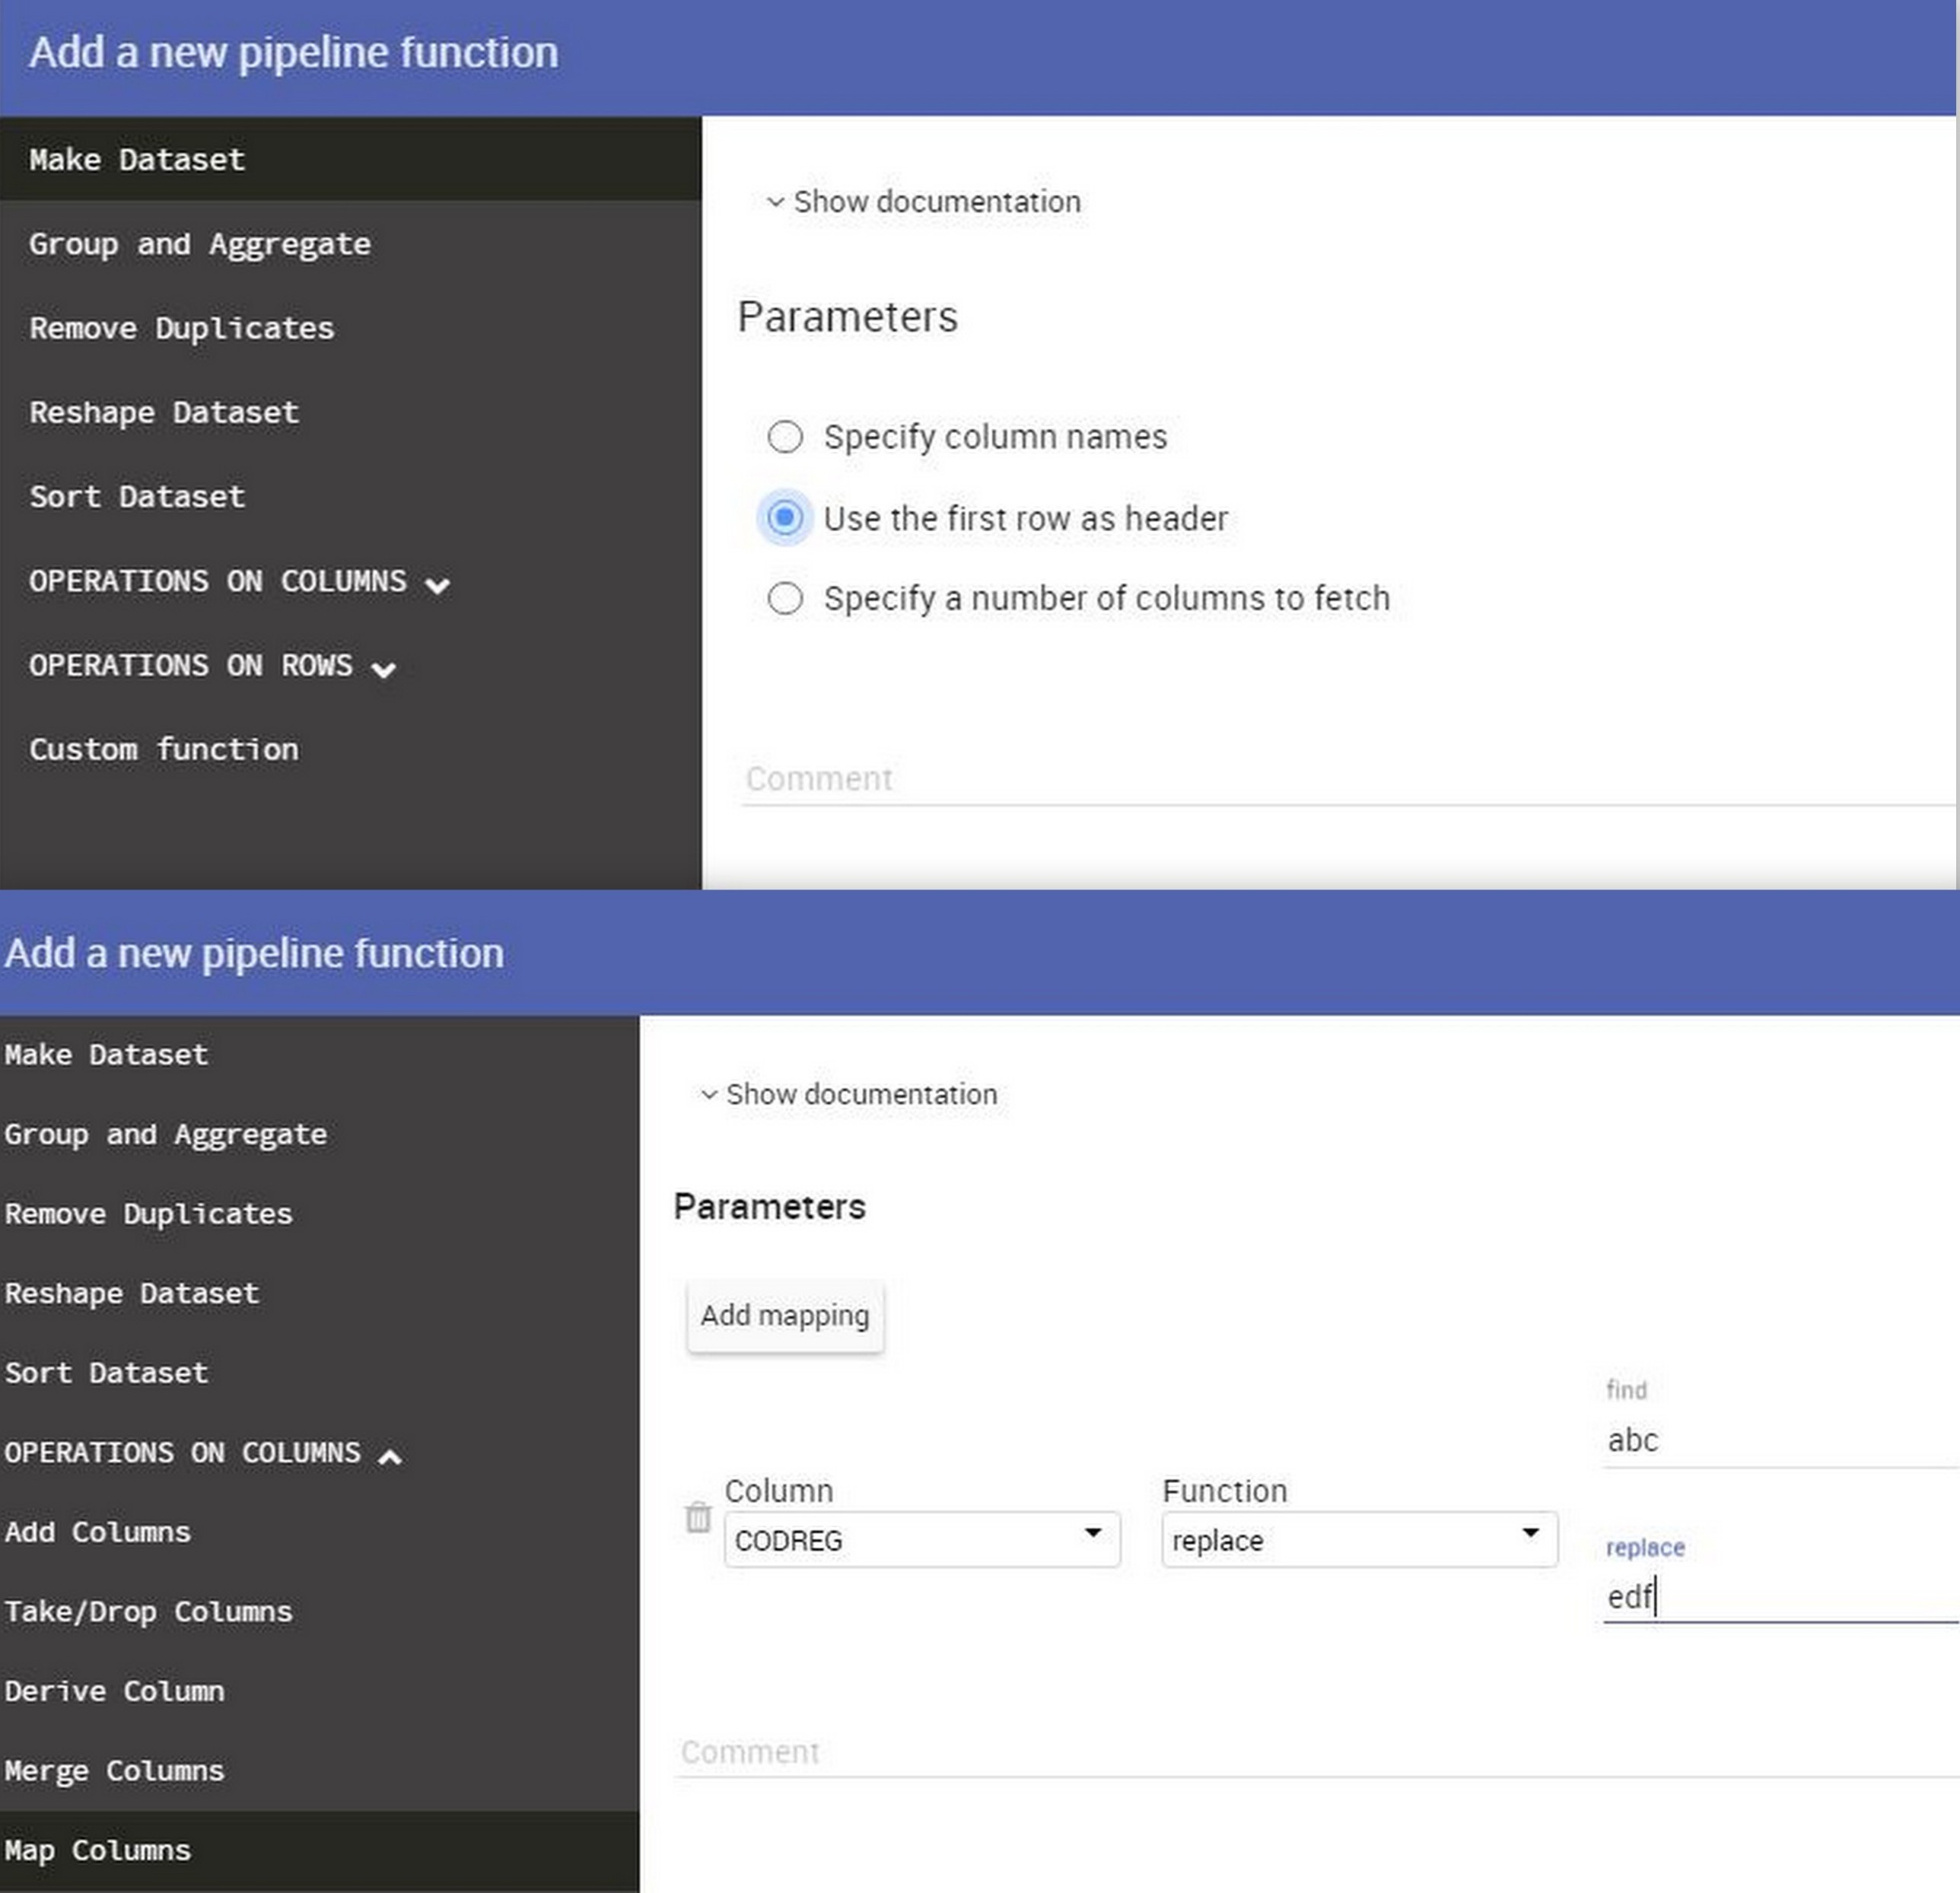
\includegraphics[width=38em]{./Figures/userinteraction}
	\begin{figure}[htbp]
    \caption{Grafterizer's interactive interface to create data cleaning pipelines}
    \label{fig:datacleaning}
	\end{figure}
\end{center}
The in-built script generator of Grafterizer converts user's input to a corresponding transformation pipeline command implicitly.  
\begin{center}
	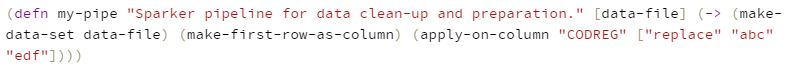
\includegraphics[width=38em]{./Figures/code-generated}
	\begin{figure}[htbp]
    \caption{Equivalent transformation pipeline script generated in Clojure}
    \label{fig:codegenerated}
	\end{figure}
\end{center}
This avoids unnecessary learning time and human errors in data preparation. Hence, Grafterizer is better suited than the other tools in terms of a complete interactive user interface that enables quicker data preparation.
\subsection{Interactivity and near-real-time response}
Provided that the treated data is large, a sample of data is created with the inputs of user to do interactive transformation. Since we consider incremental iterative transformations of large volume of data, with near-real-time response to have effective user interaction, sampling is essential.  Also, due to iterative transformation, the data being processed changes rapidly. This requires effective disposal of objects and garbage collection. For instance, Wrangler comparably performs slower due to lack of efficient object handling and leads to a longer response time when the tool is used continuously for longer period. It was noticeable, when larger data is loaded in Wranger\cite{2011-wrangler}, that the system took more than 15 seconds just to add a transformation pipeline in user interface, which later resulted in hindering user interaction holding user to wait for performing next data cleaning activity. Comparably, Grafterizer is very effective in terms of interactivity and near-real-time responsiveness since interactive transformation is efficiently performed on sample data and utilizing perfect garbage collection of under-lying system.
\section{Performance Evaluation Aspects}
In this section we evaluate the performance of implemented prototype in different experiments analyzing some critical aspects of proposed system, to draw conclusions of solution's viability from the results.
\subsection{Single Node Analysis}
\label{singlenode}
One of the important aspects Sparker gives is performing parallel execution of data preparation. Despite the system is hosted in a single machine, by exploiting in-memory computing and parallelization, Sparker can process large data faster than traditional processing applications. To analyze the performance of Scalable-graftwerk (using Sparker) in a single node, we created following sets of experiments that compares the performance of traditional processing application Graftwerk (using Grafter) and free-desktop version of Trifacta's Wrangler\footnote{https://www.trifacta.com/trifacta-wrangler/}. 

\textbf{Experimental setup}

Tests were conducted by sending HTTP requests to Scalable-Graftwerk and Graftwerk with corresponding data and transformation pipeline scripts then measuring the execution time taken to process the requests, whereas time elapsed to generate results from a pre-built transformation was recorded using stop watch in Wrangler which was installed as a standalone desktop application. Measuring execution time of pre-built transformation allows us to analyze the actual execution time, without considering the time taken to create transformation pipeline using UIs of these systems to come to a precise conclusion. All three systems were tested on same host computer with the following specifications:
\begin{itemize}
\item CPU - Intel Core i5-3210M CPU - 2.5 GHz - 4 cores
\item RAM - 8GM 
\item Operating System - Microsoft Windows 10 Home (64- bit Operating System, x64-based processor)
\end{itemize}
Scalable-Graftwerk was deployed using local-mode with \textit{ spark.master = local[*]} configuration. This allows Spark to utilize maximum parallelization of host computer.  

\textbf{Experiments and Results}

Experiments were performed on data of casualties from road accidents during 2005-2014 in Great Britain from Road Safety Data published on open data portal of Great Britain\footnote{https://data.gov.uk/dataset/road-accidents-safety-data}. The data is originally 94.9 MB, which is sampled into number of samples of smaller size and merged to create bigger data for the evaluation in the range of 9.3 MB to 120.7 MB. In total, we performed 12 experiments with different sized data-sets. A sample data transformation was created to perform data profiling, to remove two unnecessary columns and to do some word transpositions on specific columns. Equivalent transformation scripts were created for Scalable-Graftwerk, Grafwerk and Wrangler using corresponding interfaces. 
\begin{center}
	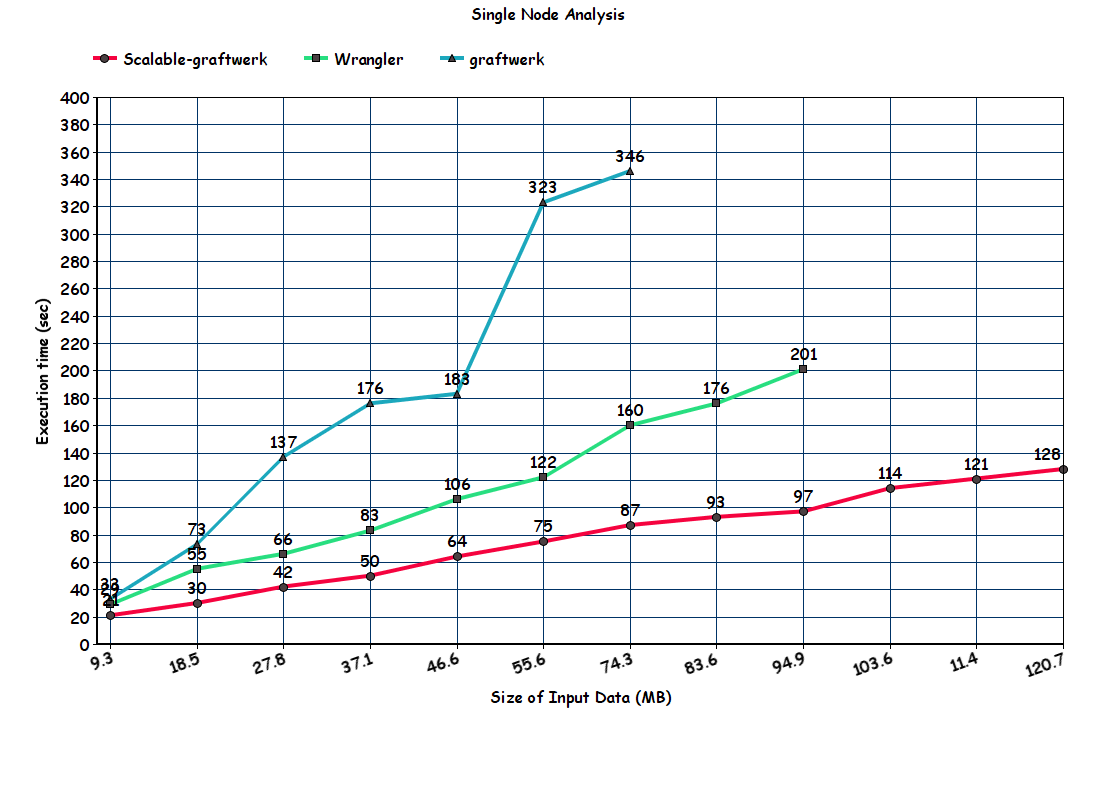
\includegraphics[width=38em]{./Figures/single-node}
	\begin{figure}[htbp]
    \caption{Single node analysis}
    \label{fig:singlenode}
	\end{figure}
\end{center}
Figure \ref{fig:singlenode} shows the execution time elapsed to process same data transformation on different sized data. Execution time of Wrangler and Scalable-graftwerk linearly increasing with the size of data.Wrangler has almost double the amount of execution time compared to Sparker,while Wrangler couldn't process data which is more than 100 MB in size. The maximum amount of data size that can be processed in Scalable-grafter converges to its allocated memory in local-mode. Whereas, Graftwerk with Grafter performed very slow compared to other two systems with roughly four times longer execution time than Sparker.

Another important fact to notice is Graftwerk, required a compulsory increase of heap size to process larger files. Figure \ref{fig:heapsize} shows the amount of heap size in GB, which was allocated during each experiments in all three systems. It is obvious to notice that, Grafter consumes large amount of heap memory to perform cleaning operations as a pipeline. When the process hits the allocated heap memory, the process stays idle or throws GarbageCollector(GC) GC overhead limit exceeded Exception. The reason can be since Grafter uses Clojure, which uses immutable objects, lack of effective garbage collection could have resulted in huge growth of heap memory to hold created data objects. It is noticeable that Graftwerk requires almost additional 1GB to process every 10 MB of input data, which is not feasible to process very large volumes of data. We could not continue the experiment for an input data which is more than 75 MB on Graftwerk. On the other hand, Scalable-graftwerk was allocated 1GB of memory and Wrangler used 1GB of memory throughout the experiments
\begin{center}
	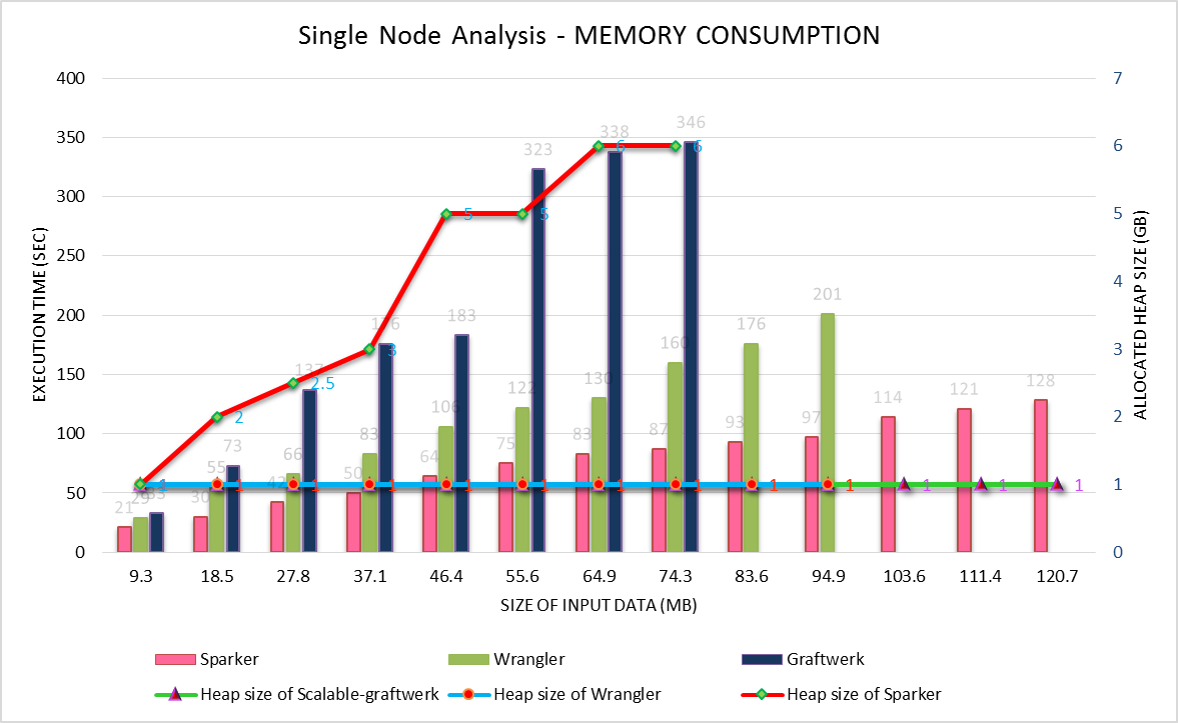
\includegraphics[width=38em]{./Figures/heapsize2}
	\begin{figure}[htbp]
    \caption{Heap sized used for Single Node Analysis}
    \label{fig:heapsize}
	\end{figure}
\end{center}
With the above experiments, it is safe to conclude that Scalable-graftwerk performs better in terms of capacity to process large files and faster execution time. 
\subsection{Cluster Analysis}
\textbf{Experimental setup}

The main goal of this thesis is to provide a scalable data preparation as a service. Thus, it is vital to investigate the scalability of proposed system. In order to measure the scalability of the system, we conducted few sets of experiments on Scalable-grafter. Scalable-grafter was deployed on a cluster using \textit{spark-submit}\footnote{http://spark.apache.org/docs/latest/submitting-applications.html} The cluster is managed by YARN resource manager\footnote{http://hadoop.apache.org/docs/current/hadoop-yarn/hadoop-yarn-site/YARN.html} in \textit{yarn-client mode} which suits interactive style of commands\footnote{http://blog.cloudera.com/blog/2014/05/apache-spark-resource-management-and-yarn-app-models/}. The cluster consists a master-slave architecture with following specifications:
\begin{itemize}
\item Master  Node : 	Intel Core i7 5820K 3.3GHz, 4 CPU Cores, 15 GB of RAM, 512GB of SATA SSD, Ubuntu 14.04 LTS
\item Worker Nodes : 4 x (Intel Core i7 5820K 3.3GHz, 12 CPU Cores, 64 GB of RAM, 480GB NVME SSD, 6*3 TB HDD, CentOS 7)
\end{itemize}
\begin{center}
	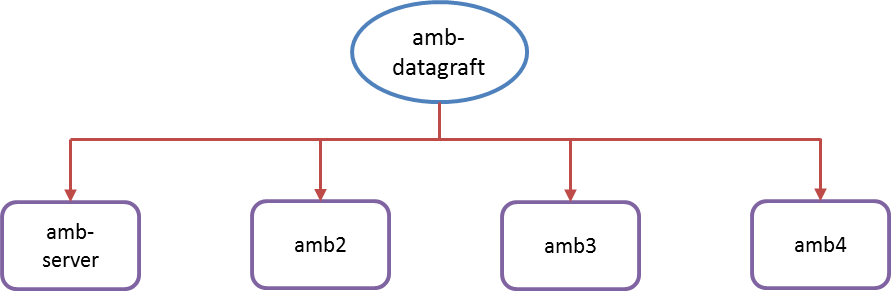
\includegraphics[width=38em]{./Figures/cluster}
	\begin{figure}[htbp]
    \caption{Structure of cluster}
    \label{fig:cluster}
	\end{figure}
\end{center}
Figure \ref{fig:cluster} depicts how the our test bed was setup.   two main parameters that can influence spark's performance are memory and CPU. Network I/O and Disk also affect Spark application's performance. However, YARN or Spark don't actively manage them till now. They are considered irrelevant in our experiments since we do not consider network provisioning time when creating SparkContext and reconcile data for these experiments. The performance of a Spark application like Scalable-graftwerk can be analyzed by tuning allocated memory and CPU. Focusing on scalability of the application, we decided to change the CPUs allocated to application and track performance accordingly.

\textbf{YARN Execution Model on a Cluster}

A Spark application consists of a single-driver process and a set of executor processes scattered across nodes on the cluster. The driver process  is responsible for the high-level control flow of work that needs to be done. The executor processes are responsible for executing this work, in the form of tasks. When a Spark application is submitted using park-submit using \textit{yarn-client} mode, a central master application request YARN resource manager for resource containers. YARN Manager informs master application with available resources according to request. The client's master application directly communicates containers to schedule jobs. 
\begin{center}
	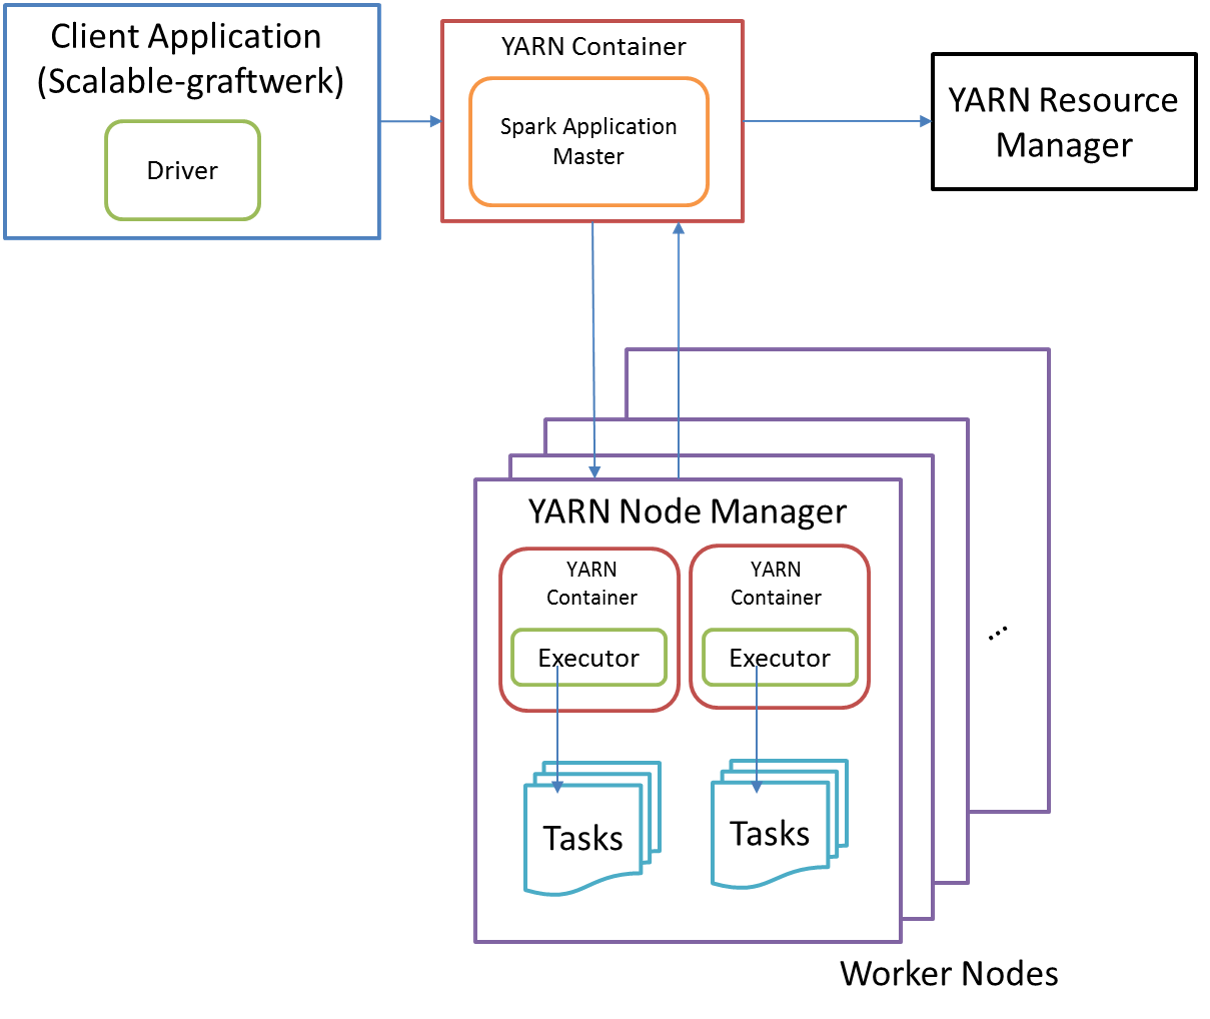
\includegraphics[width=33em]{./Figures/scalable-graftwer-in-yarn-cluster}
	\begin{figure}[htbp]
    \caption{Scalable-graftwerk's execution model on a YARN Cluster}
    \label{fig:yarn-cluster-model}
	\end{figure}
\end{center}
A Spark application can be manually tuned with respect to CPU by changing following properties
\begin{itemize}
\item Number of executors : 	An executor is a single JVM instance on a node that serves a spark application. An executor can run multiple tasks concurrently. Every executor has equal number of tasks and fixed amount of heap size
\item Number of cores used in a driver: Number of concurrent tasks an executor can run
\item Number of cores used in an executor:  Number of concurrent tasks an driver can run
\end{itemize}
These can be easily tuned by modifying spark configuration of the deployment to analyze the performance. 

\textbf{Experiments and Results}

All the experiments mentioned below are performed on Price Paid Data which contains information on all residential property sales in England and Wales that are sold for full market value and are lodged with Land Registry for registration\footnote{https://www.gov.uk/government/statistical-data-sets/price-paid-data-downloads}. The data-set contains information from 1st of January 1995 to the end of April 2016, that is 3.5 GB in size. We created a sample transformation that can load the file and make a data-set by using the first row values as column headers. The experiment was performed by sending HTTP Requests with generated data cleaning scripts and location of input file in HDFS. Figure \ref{fig:sample-pipeline} shows the cleaning script generated by integrated Grafterizer. 
\begin{center}
	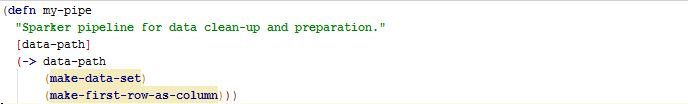
\includegraphics[width=35em]{./Figures/cluster-pipeline}
	\begin{figure}[htbp]
    \caption{Sample data cleaning script}
    \label{fig:sample-pipeline}
	\end{figure}
\end{center}
 Figure \ref{fig:spark-test-job} shows how the script generated in Figure \ref{fig:sample-pipeline} is executed in Spark. This involves 4 small tasks including fetching the first line, create a map of each line with an index and create new schema with provided logic and save the result as a CSV file in HDFS. It can be clearly seen the level of abstraction Scalable-graftwerk provides to execute Spark jobs eases the efforts of data workers.
\begin{center}
	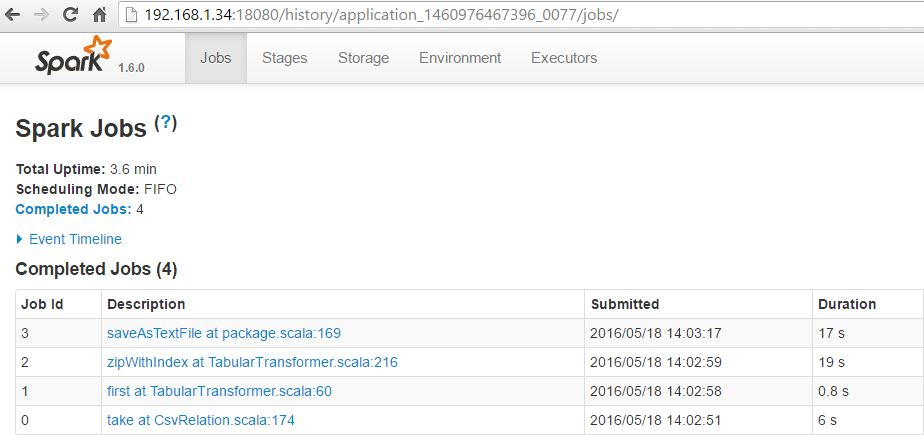
\includegraphics[width=38em]{./Figures/spark-job}
	\begin{figure}[htbp]
    \caption{Spark job of tested data cleaning pipeline}
    \label{fig:spark-test-job}
	\end{figure}
\end{center}
All the experiments below were executed with 
\begin{itemize}
\item Driver-memory : 4GB
\item Executor memory : 10GB
\item Default parallelism 
\end{itemize}
\subsubsection{\textbf{Scalability of Scalable-graftwerk}}
\label{scalability-exp}
The first experiment was conducted by deploying the application with a different number of executors with fixed number of driver cores and fixed number of executor cores. In this experiment we chose to use 2 driver cores and 2 executor cores per executor. We changed the number of executors from 1 to 20 to analyze the impact of number of executors in our application's performance. 
\begin{center}
	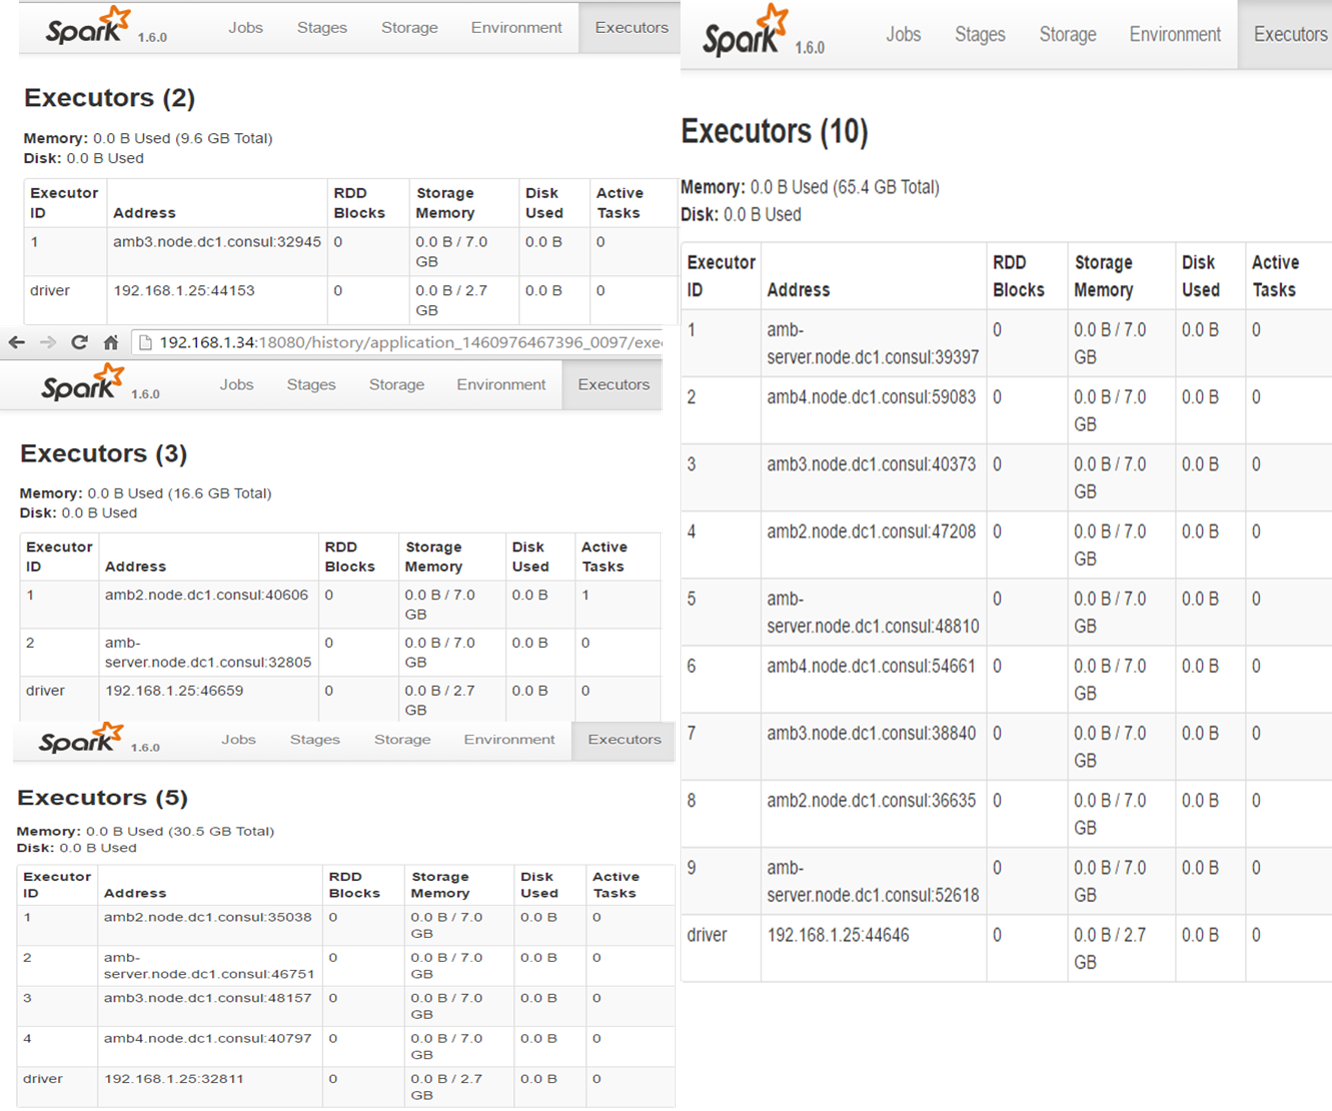
\includegraphics[width=35em]{./Figures/scale}
	\begin{figure}[htbp]
    \caption{Scalability of Scalable-graftwerk on distributed nodes}
    \label{fig:scale}
	\end{figure}
\end{center}
Figure \ref{fig:scale} shows that Scalable-graftwerk can automatically scale-out on different nodes when number of executors are changed. This lets the application to utilize the resources available on a cluster
\begin{center}
	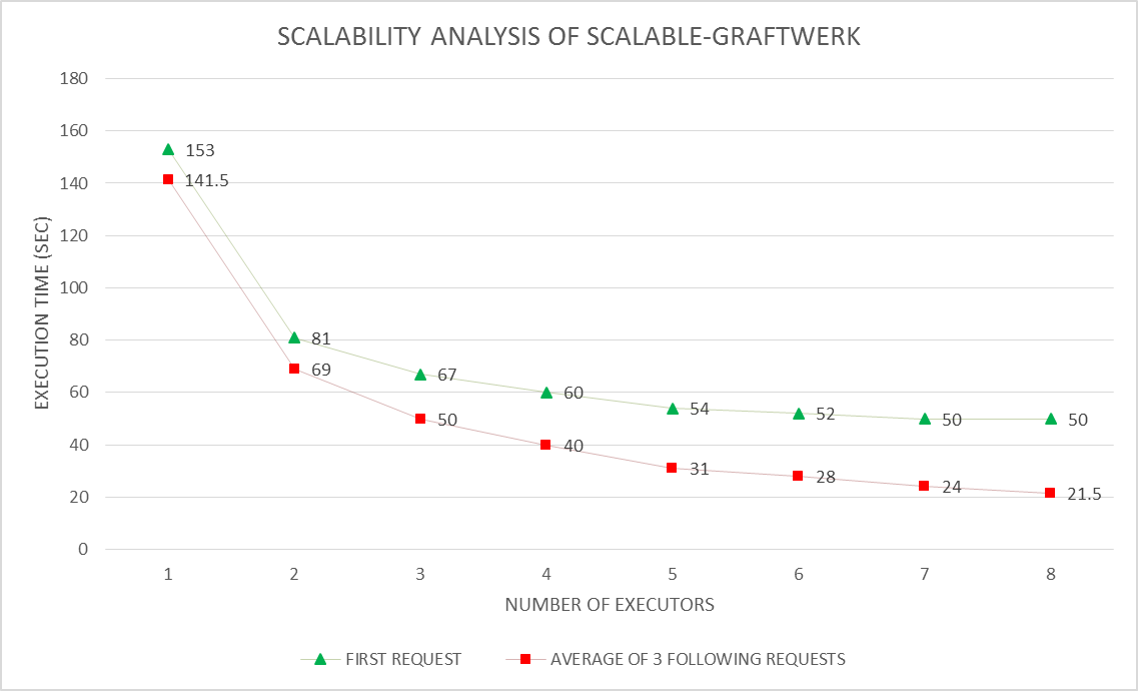
\includegraphics[width=38em]{./Figures/executors2}
	\begin{figure}[htbp]
    \caption{Scalability analysis of Scalable-Graftwerk}
    \label{fig:executors}
	\end{figure}
\end{center}
We noticed that there is a significant difference between execution time of the first request after a SparkContext is initialized and requests follow the first request, while the difference between following request were significantly small (0 -2 seconds). Reasons for this difference can be initialization of tasks in background that are required for execution of a job. Since, we are providing Scalable-graftwerk as a service, the execution time of first request seldom impacts on application performance, since the service is expected to be available when a user starts a data preparation process. We focus more on the performance on interactive, and iterative operations. Thus, we recorded the execution time of first request and average of 3 following request for this set of experiments. Figure \ref{fig:executors} shows the execution time elapsed for different number of executors. The main observations we noticed from these experiments are, 
\begin{itemize}
\item Execution time of a job is improved with maximum difference of 125 seconds (141.5 to 15.5) with 1 to 20 executors. 
\item Performance of application increases exponentially for both first request and average of following request till a minimum execution time of executed job is reached ( met with 8 executors ).  
\item Execution time of first request starts to increase from 9 executors (after minimum required execution time is met) and remains almost unchanged after 15 executors.
\item Execution time of average of following requests is nearly unchanged with decrease of maximum of 5 seconds from 9 executors to 20 executors
\end{itemize}
It can be clearly seen that performance of the application increases till a minimum threshold execution time is reached. When more executors are provided, it creates multiple virtual cores that can equally execute a job in parallel. The more executors are allocated, the less work-load is shared per executor. However, parallelism of tasks plays a significant role in Spark application's execution time, which we don't focus in this experiment. We notice that a job lasts at least for a minimum amount of time, regardless of increase of executors with unchanged parallelism. We refer this as the minimum execution time of a Spark job for a given parallelism. Once the minimum threshold of execution time of a job is reached execution time of a first request increases. When more executors are used it requires initialization and coordination of background tasks in more executors, while the process requires at least a minimum amount of execution time. This reasons the behavior of execution time of first request. Through this experiment we conclude that Scalable-graftwerk is scalable with default parallelism until the minimum execution time of corresponding Spark job is reached. 
 
\subsubsection{\textbf{Concurrent execution of multiple tasks}}
Apart from scalability experiment discussed in Section \ref{scalability-exp} , we conducted another experiments to analyze whether we can  improve the performance of Scalable-graftwerk further. We set up more sets of experiments by changing the number of cores allocated for each executors from 1 to 12, with fixed number of executors and fixed number of driver cores. 

To analyze the behavior of concurrent task execution, we conducted 3 sets of experiments with 2, 5  and 7 executor instances and 2 cores for driver process. Since the average execution time of requests after the first request represents application's performance than execution time of first request after a SparkContext is initialized, we recorded the average execution time of 3 requests after the first request of an initiated context.
\begin{center}
	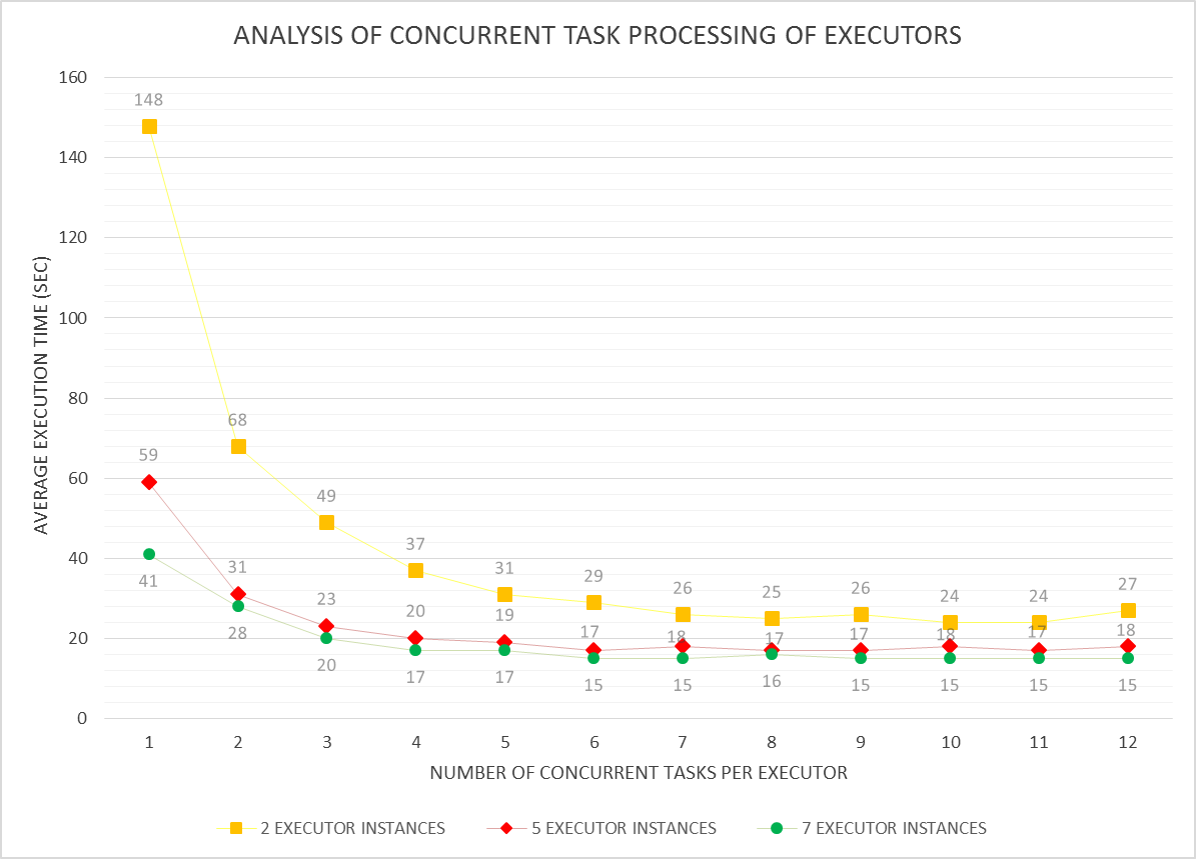
\includegraphics[width=38em]{./Figures/executor-cores2}
	\begin{figure}[htbp]
    \caption{Analysis of concurrent task processing of executors}
    \label{fig:executor-cores}
	\end{figure}
\end{center}
Figure \ref{fig:executor-cores} illustrates the observations of these experiments.  It is clear that, there is an exponential growth of performance from 1 core to 6 cores per executor. From 6 executors to 12 executors the performance is not significantly improved. It is rather unchanged with small differences ( 2 seconds ). The reason behind this behavior is HDFS has some performance limitations of concurrent task processing. When more than 5-6 concurrent tasks are executed on an executor process, the performance of the application is not improved as expected, since an overhead of processing too many concurrent tasks are introduced on HDFS. It is wise to keep the number of concurrent tasks (executor-cores per executor) below this limit for the optimal performance of this application.  

Moreover, the improvement in execution time increases with indirect-proportion of number of executors. Further it can be clearly seen, the impact of having more executors improve performance of the application, regardless of parallelization of concurrent tasks per executor. This behavior assures the claim made from previous experiment in Section \ref{scalability-exp}. 

As mentioned earlier, the other parameter that can be tuned on a Spark application is number of driver-cores. We didn't conduct any experiments to study behavior of driver-cores, since we focus on scalability and parallization of distributed executors, whereas driver process always run on a single machine. 

Overall, through all experiments mentioned in this section, Scalable-graftwerk can scale-out with more executors according to the cluster and number of executors requested. It can improve the performance until the minimal execution time for given parallelism is reached. Further, Scalable-graftwerk's performance can further be improved by having 5-6 executor cores per executor.  


